%% ============================================================================
%% Court Vision AI -- IEEE conference paper (Overleaf-ready)
%% Compile with pdfLaTeX (Overleaf default); bibliography with BibTeX (refs.bib).
%% ============================================================================
\documentclass[conference]{IEEEtran}
\IEEEoverridecommandlockouts

\usepackage{cite}
\usepackage{amsmath,amssymb}
\usepackage{graphicx}
\usepackage{booktabs}
\usepackage{url}
\usepackage[hidelinks]{hyperref}

\begin{document}

\title{Court Vision AI: Retrieval-Grounded, Citation-Enforcing Generative AI for Indian Legal Case Preparation}

\author{
\IEEEauthorblockN{Aditya Chauhan, Pranita Bhortakke, Binoy Chhatwani, Vanshika Keshwani}
\IEEEauthorblockA{Department of Information Technology\\
Vivekanand Education Society's Institute of Technology, Mumbai, India\\
\{email1, email2, email3, email4\}@ves.ac.in}
\and
\IEEEauthorblockN{Dr. Asma Praveen}
\IEEEauthorblockA{Department of Information Technology\\
Vivekanand Education Society's Institute of Technology, Mumbai, India\\
guide.email@ves.ac.in}
}

\maketitle

%% ----------------------------------------------------------------------------
\begin{abstract}
Preparing a criminal or civil matter in India requires advocates and law students to read long judgments, First Information Reports and witness statements, and then to assemble chronologies, cross-examination questions and supporting precedents by hand. General-purpose large language models (LLMs) can assist with this reading, but they frequently invent facts and citations, and practical systems built on rate-limited LLM services usually show the model only the beginning of a long record. We present Court Vision AI, a web platform that grounds six case-preparation features---document chat, case summary, evidence graph, virtual courtroom, trial-preparation brief and precedent research---in the user's own case documents. Its core technique, CV-RAG, splits the record into page-tagged passages, ranks them with Okapi BM25 and supplies only the most relevant passages to the LLM, together with explicit rules to cite pages and to decline when the answer is absent. On a set of 42 questions built from a 20-page Supreme Court judgment, CV-RAG handled all 42 correctly, compared with 34 for the platform's original truncated design and 11 for the same LLM without documents ($p=0.008$ and $p<0.001$, McNemar's test), while sending 60\% fewer prompt tokens. A nested-object recovery method also restored usable evidence graphs from all cut-off LLM replies, on which every earlier parser failed.
\end{abstract}

\begin{IEEEkeywords}
Legal AI, large language models, retrieval-augmented generation, BM25, hallucination, knowledge graph, Indian law
\end{IEEEkeywords}

%% ----------------------------------------------------------------------------
\section{Introduction}
Indian courts carry a heavy backlog, and much of an advocate's preparation time is spent reading. A single matter may involve a judgment of twenty or more pages, an FIR, a charge-sheet, medical reports and several depositions. From these, the advocate must reconstruct the sequence of events, identify the witnesses and the inconsistencies between their statements, frame cross-examination questions, locate binding precedents and rehearse oral arguments. Law students and junior advocates carry the same burden with less experience and, often, without access to paid research databases.

Large language models appear well suited to this work, but their tendency to produce fluent yet false statements---hallucination---is well documented~\cite{ji2023survey}. When asked verifiable questions about US federal cases without access to the source documents, public LLMs answered incorrectly in 58--88\% of cases~\cite{dahl2024}. Even commercial legal research tools that retrieve documents before answering were found to hallucinate in 17--33\% of responses~\cite{magesh2025}. In legal practice, an invented date, FIR number or precedent can mislead a court and prejudice a client.

A further, more practical problem arises when such assistants are deployed on affordable LLM services. Free tiers restrict the number of tokens that can be processed per minute, so systems commonly truncate the case record. The first version of our own platform sent only the first 18,000 characters of a case to the model; for the 72,720-character judgment in \emph{Jacob Mathew v. State of Punjab}~\cite{jacobmathew2005} used in our evaluation, this is only 24.8\% of the text. Questions about later pages therefore could not be answered, and the model's polite statement that the information was ``not available'' concealed the limitation from the user.

This paper makes the following contributions:
\begin{itemize}
\item \textbf{Court Vision AI}, a full-stack platform for Indian legal case preparation with six features grounded in the user's documents.
\item \textbf{CV-RAG}, a page-tagged BM25 retrieval layer with citation and refusal rules that operates within an 8,000 tokens-per-minute budget.
\item A \textbf{self-growing precedent library} that stores each uploaded judgment together with the authorities it cites, using the citations printed in the judgment.
\item A \textbf{nested-object recovery method} that extracts usable structured data from LLM replies cut off by the output limit.
\item A \textbf{controlled evaluation} on 42 questions with known answers, including deliberately unanswerable questions, with paired significance tests.
\end{itemize}

%% ----------------------------------------------------------------------------
\section{Related Work}
\textbf{Legal hallucination.} Dahl et al.~\cite{dahl2024} profiled the errors of ChatGPT~3.5, PaLM~2 and Llama~2 on questions about US federal cases and found that the models not only answered incorrectly most of the time but also accepted false premises and could not recognise their own errors. Magesh et al.~\cite{magesh2025} conducted a pre-registered study of retrieval-based commercial tools (Lexis+ AI, Westlaw AI-Assisted Research and Ask Practical Law AI) and showed that retrieval reduces but does not remove hallucination, in part because systems sometimes cite real authorities for propositions those authorities do not support.

\textbf{Indian legal NLP.} The ILDC corpus of about 35,000 Supreme Court cases~\cite{malik2021ildc} enabled judgment prediction with explanation, although model explanations agreed poorly with expert explanations. InLegalBERT~\cite{paul2023inlegalbert} showed that continued pre-training on Indian judgments improves statute identification, rhetorical segmentation and judgment prediction. IL-TUR~\cite{joshi2024iltur} assembled eight tasks across English and nine Indian languages and found current models well below expert level. LegalBench~\cite{guha2023legalbench} evaluated 20 LLMs on 162 US legal reasoning tasks with short inputs. These efforts concentrate on classification and prediction; none measures question answering or refusal over a practitioner's own long case file.

\textbf{Retrieval and simulation.} Retrieval-augmented generation (RAG)~\cite{lewis2020rag} conditions an LLM on retrieved passages, and GraphRAG~\cite{edge2024graphrag} builds an LLM-extracted entity graph for corpus-level summarisation, assuming well-formed model output. AgentCourt~\cite{chen2025agentcourt} simulates court proceedings with evolving LLM lawyer agents under Chinese law. To our knowledge, no prior work grounds question answering, evidence mapping and courtroom practice in a user's own Indian case record while operating within the limits of an affordable LLM service; this is the gap that Court Vision AI addresses.

%% ----------------------------------------------------------------------------
\section{System Overview}
Court Vision AI is a three-tier web application (Fig.~\ref{fig:arch}). The front end is built with Next.js and React; the server uses FastAPI with SQLAlchemy over PostgreSQL; and LLM inference is provided by Groq, using \texttt{openai/gpt-oss-120b} with two smaller fallback models. Uploaded PDF files are checked for extension, size (up to 50~MB) and PDF signature, stored, and processed in a background task that extracts their text with PyMuPDF.

The platform offers six features. \emph{Case Intelligence} answers questions about a case with references to the source document. \emph{Case Snapshot} produces a structured summary of issues, facts, dates, evidence, weaknesses and next steps. \emph{Evidence Graph} displays persons, organisations, facts, evidence and dates together with labelled relationships. \emph{Virtual Courtroom} lets the user argue a case in four phases before an AI judge whose temperament can be strict, inquisitive or balanced, against an AI opposing counsel, and ends with a verdict and a performance scorecard. \emph{Trial Prep \& Brief Generator} produces a date-wise chronology, a cross-examination question bank and a seven-section synopsis. \emph{Legal Precedents} searches a precedent library and supplements it with labelled AI suggestions.

All features rely on three shared services: a retrieval service that creates and ranks page-tagged passages, an LLM service that handles model fallback, rate-limit waits, request sizing and output repair, and a precedent service that builds and searches the precedent library.

\begin{figure}[t]
\centering
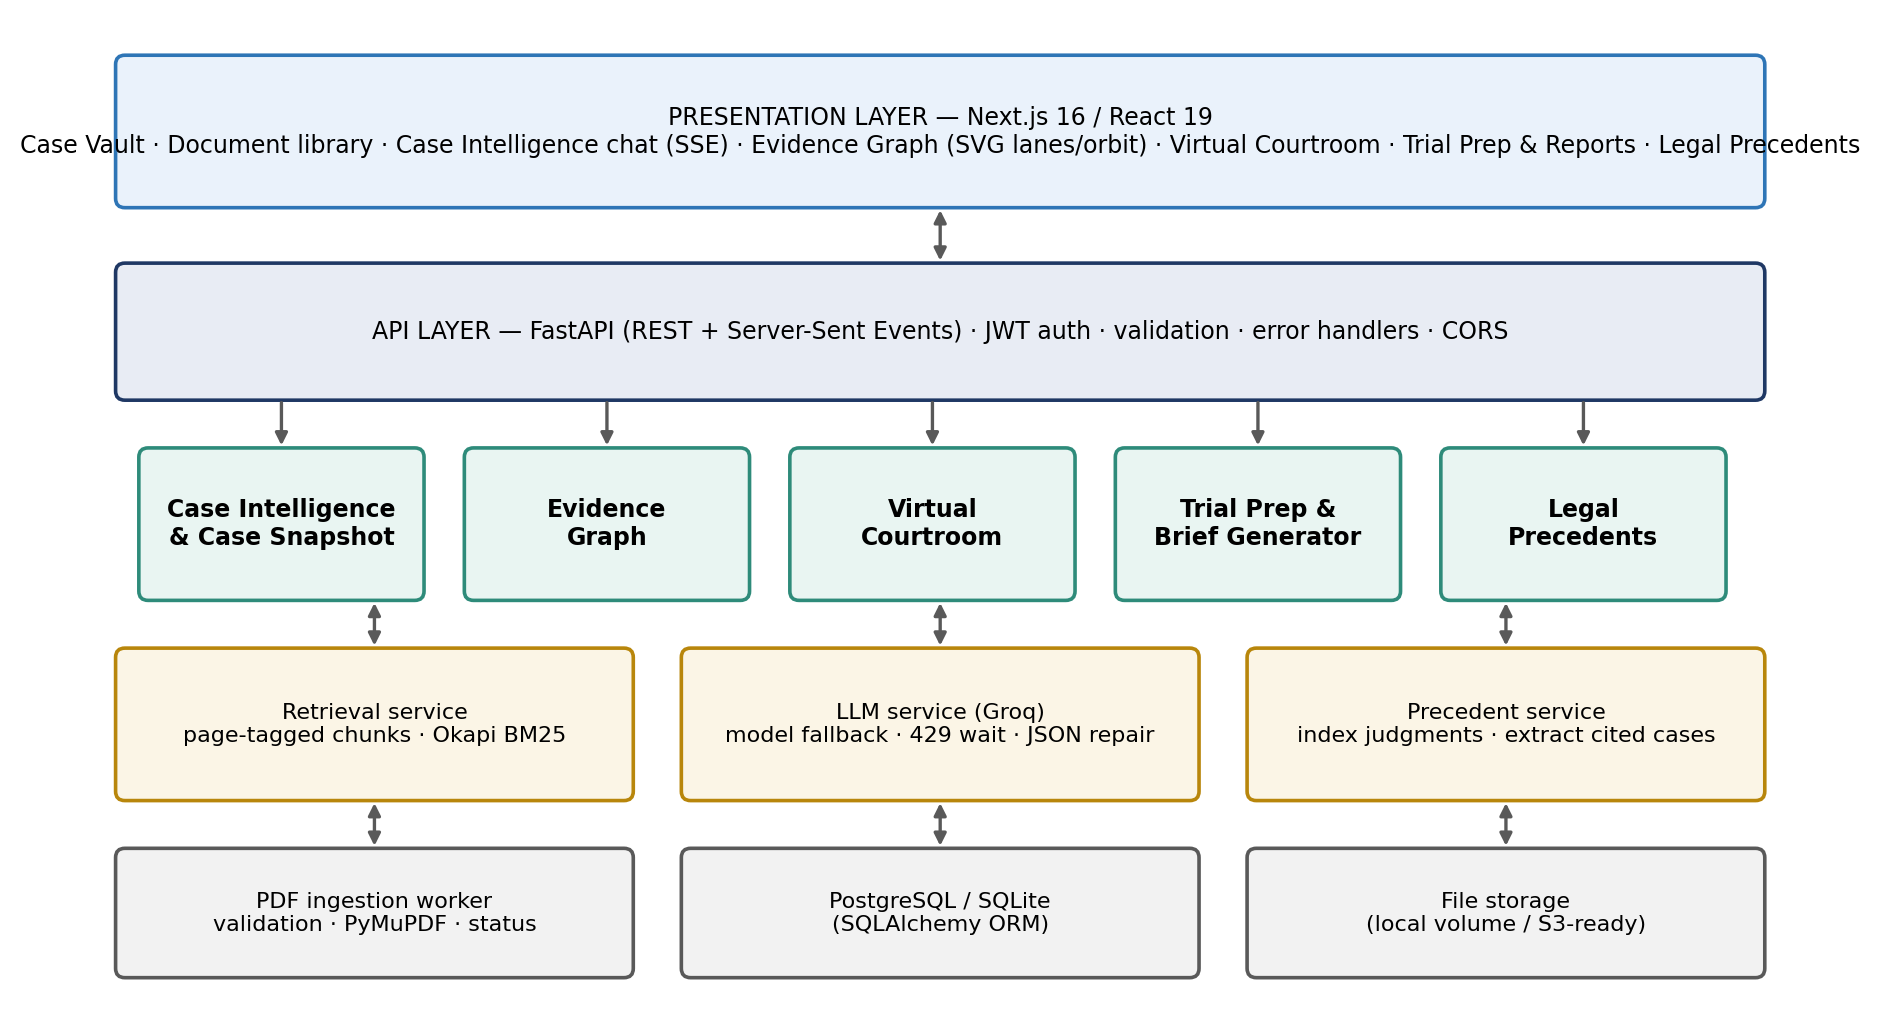
\includegraphics[width=\linewidth]{figures/block_diagram.png}
\caption{Architecture of Court Vision AI: presentation, API, features, shared services and data layer.}
\label{fig:arch}
\end{figure}

%% ----------------------------------------------------------------------------
\section{Proposed Method}

\subsection{CV-RAG: Page-Tagged Passage Retrieval}
Each document is read page by page; running headers, footers, URLs and page numbers are removed, and the text of each page is divided into 1,000-character chunks with a 200-character overlap. Every chunk carries its document name and page number. For a query $q$, each chunk $d$ is scored with Okapi BM25~\cite{robertson2009bm25}:
\begin{equation}
\mathrm{score}(q,d)=\sum_{t\in q}\mathrm{IDF}(t)\,\frac{f(t,d)\,(k_1+1)}{f(t,d)+k_1\left(1-b+b\,\frac{|d|}{\mathrm{avgdl}}\right)},
\label{eq:bm25}
\end{equation}
\begin{equation}
\mathrm{IDF}(t)=\ln\!\left(1+\frac{N-n(t)+0.5}{n(t)+0.5}\right),
\end{equation}
where $f(t,d)$ is the frequency of term $t$ in $d$, $|d|$ the chunk length, avgdl the mean chunk length, $N$ the number of chunks and $n(t)$ the number of chunks containing $t$; we use $k_1=1.5$ and $b=0.75$. The top-$k$ chunks ($k=6$ for question answering) are restored to document order and inserted into the prompt as ``[document, p.~N] text''. Two rules are added to the system prompt: every factual claim must cite its page, and when the passages do not contain the answer the model must reply that the information is not available in the uploaded documents (Fig.~\ref{fig:cvrag}). BM25 requires no training or GPU, and ranking 91 chunks takes well under a millisecond.

\begin{figure}[t]
\centering
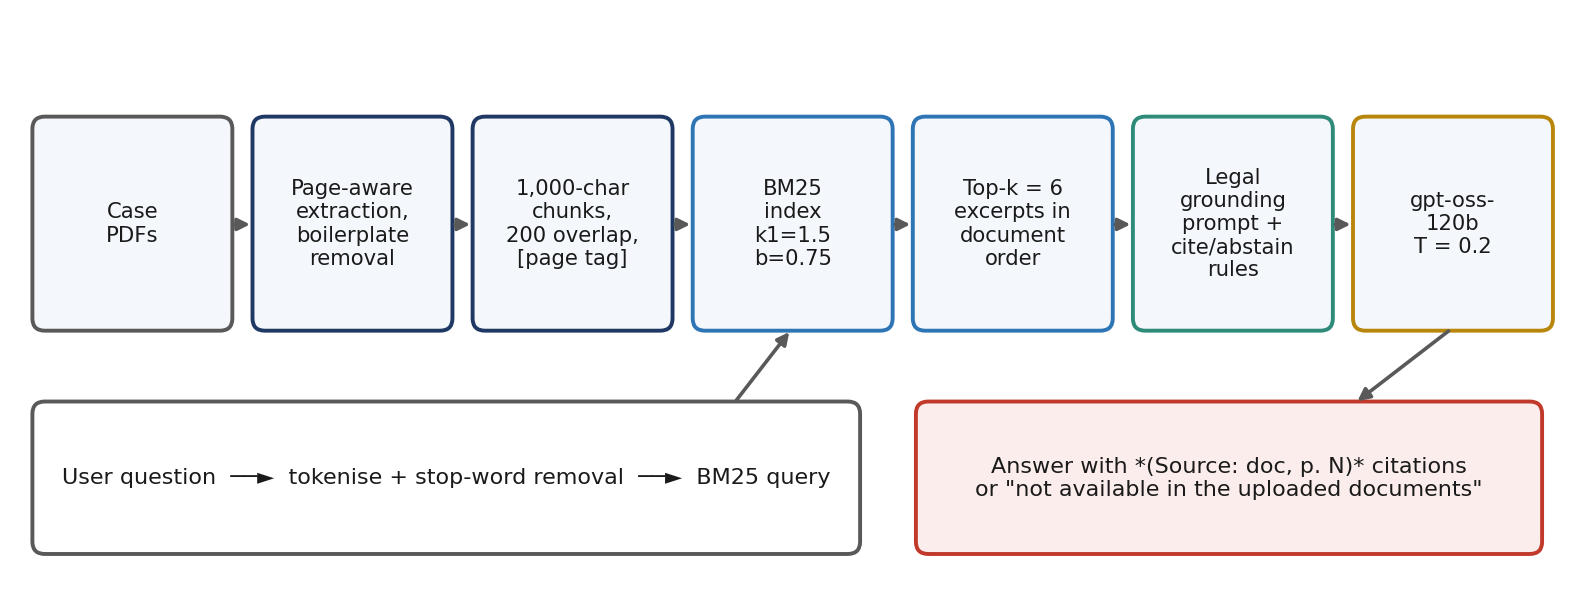
\includegraphics[width=\linewidth]{figures/fig_cvrag.png}
\caption{CV-RAG pipeline: page-aware extraction, chunking, BM25 ranking and grounded prompting with citation and refusal rules.}
\label{fig:cvrag}
\end{figure}

\subsection{Precedent Library}
When a judgment finishes processing, it is fingerprinted with SHA-256 so that the same judgment uploaded to several cases is stored once. The LLM extracts its metadata---title, citation, court, bench, ratio decidendi, statutes and keywords---from the opening and closing pages; if this fails, title, citation and court are read directly from the text with patterns. Reported citations in the body (SCC, SCR, AIR, All~ER, WLR, AC, Bom~LR and others) are then located with regular expressions, and a 260-character window on each side is sent to the LLM in batches of twelve to identify the cited case and the proposition for which it was cited. A cited case is accepted only if its citation matches the printed citation of that window and a word of its name appears in the same window, which prevents names from being paired with the wrong citation. The court is inferred from the law report. Indexing one Supreme Court judgment added 21 cited authorities with their printed citations. During precedent research, AI-suggested cases are marked as verified only when they match a library entry; suggestions for which the model cannot give a reliable citation are withheld and the user is informed.

\subsection{Evidence Graph with Duplicate Removal}
The graph prompt receives the opening and closing pages of the record together with the passages ranked highest for parties, witnesses, evidence, dates and findings (up to 10,000 characters). The model must return each real-world entity once, with all aliases, a one-line role with a page reference, and, for each relationship, a short phrase stating its legal significance. A deterministic step then normalises names by removing titles such as Dr., Shri and Smt.; merges entities whose names or aliases match, or persons whose multi-word names contain one another; redirects relationships to the surviving entity; removes self-links and duplicate links; and keeps the 28 most connected entities. Fig.~\ref{fig:graph} shows a graph produced for a maintenance case.

\begin{figure}[t]
\centering
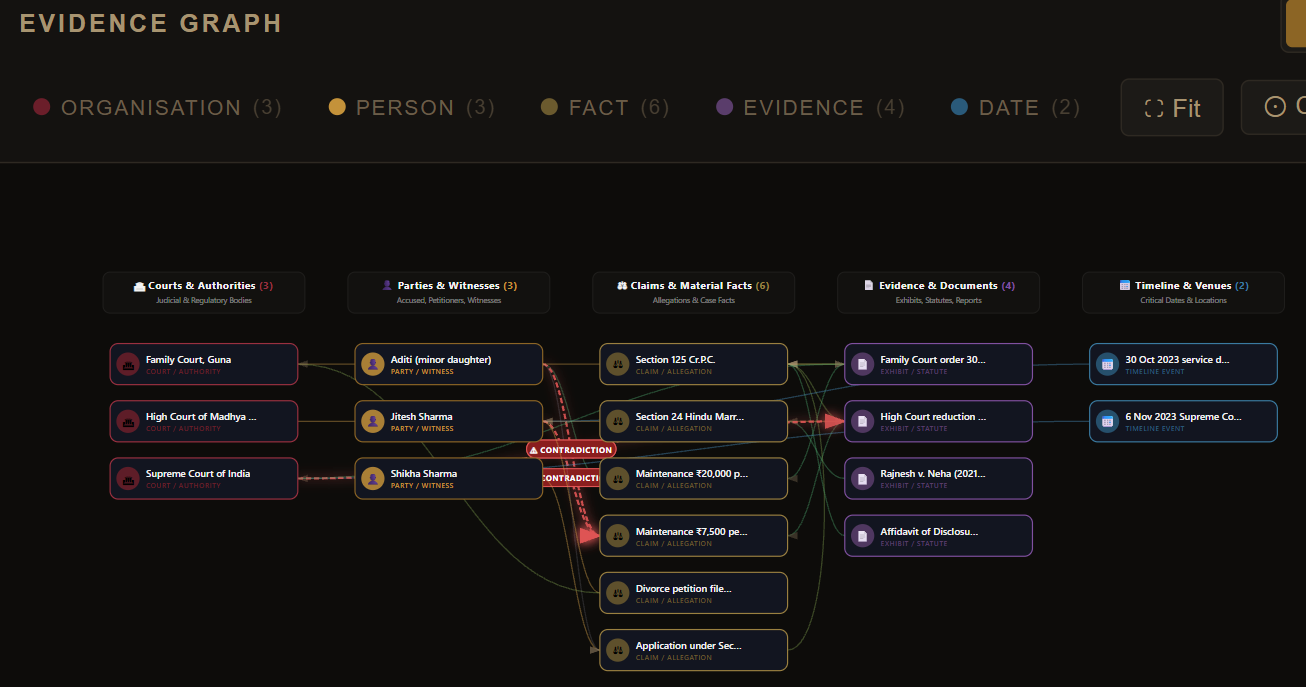
\includegraphics[width=\linewidth]{figures/evidence_graph_full.png}
\caption{Evidence graph of a maintenance case: entities in typed columns, contradictory claims highlighted.}
\label{fig:graph}
\end{figure}

\subsection{Recovering Cut-Off LLM Output}
Several features request JSON output. When a reply exceeds the output limit it is truncated, and standard parsing fails. The platform's original recovery routine collected only objects that closed at the outermost level---which never occurs when the outer object is cut off---and the trial-brief feature silently fell back to template text in that situation. Our method keeps a stack of the positions of opening braces, ignoring characters inside strings, and on every closing brace attempts to parse the enclosed text, thereby recovering every complete object at any depth. Callers retain objects of the expected shape, such as graph nodes and edges or chronology entries. In addition, when the service rejects a reply in JSON mode because of a minor syntax error, the rejected text is repaired and parsed rather than discarded.

%% ----------------------------------------------------------------------------
\section{Experimental Setup}
\textbf{Question set.} Before any system was run, we wrote 42 questions with known answers from the full text of \emph{Jacob Mathew v. State of Punjab}~\cite{jacobmathew2005}. Group~A (16 questions) can be answered from the first 18,000 characters; group~B (14) can be answered only from later pages; and group~C (12) cannot be answered from the judgment at all, such as the FIR number or the name of the duty nurse (Table~\ref{tab:groups}). Group~C tests whether a system invents facts.

\textbf{Systems.} All LLM-based systems used \texttt{openai/gpt-oss-120b} at temperature 0.2 with fallback disabled: (1) the \emph{original design}, which sends the first 18,000 characters with the platform's legal prompt; (2) \emph{CV-RAG}; (3) the \emph{LLM without documents}, given only the case name; and (4) \emph{keyword search only}, which returns the top BM25 passage without an LLM.

\textbf{Scoring.} An answer to an answerable question is correct if it contains the key fact of the known answer; for an unanswerable question, the system must decline. We report correct answers, correct declines, invented answers and wrong declines, and define \emph{handled correctly} as correct answers plus correct declines. We give Wilson 95\% intervals, McNemar's exact test~\cite{mcnemar1947} for paired outcomes and the Wilcoxon signed-rank test for latency. Experiments ran on an AMD Ryzen~5 5625U laptop against the Groq free tier (8,000 tokens per minute).

\begin{table}[t]
\centering
\caption{Examples of the three question groups}
\label{tab:groups}
\footnotesize
\begin{tabular}{p{1.1cm}p{3.8cm}p{2.4cm}}
\toprule
\textbf{Group} & \textbf{Example question} & \textbf{Expected behaviour}\\
\midrule
A (16) & On what date was Jiwan Lal Sharma admitted to the hospital? & Answer 15.02.1995 (p.~1)\\
B (14) & Which English case laid down the test for medical negligence applied in India? & Answer \emph{Bolam} (p.~6)\\
C (12) & On what date was the FIR lodged? & Decline (date not stated)\\
\bottomrule
\end{tabular}
\end{table}

%% ----------------------------------------------------------------------------
\section{Results and Discussion}

\begin{table}[t]
\centering
\caption{Results on the 42 test questions}
\label{tab:results}
\footnotesize
\setlength{\tabcolsep}{3pt}
\begin{tabular}{lcccc}
\toprule
\textbf{Measure} & \textbf{CV-RAG} & \textbf{Original} & \textbf{No docs} & \textbf{Keyword}\\
\midrule
Correct, answerable (of 30) & \textbf{30} & 22 & 8 & 26\\
\quad group A (of 16) & 16 & 16 & 2 & 14\\
\quad group B (of 14) & \textbf{14} & 6 & 6 & 12\\
Correctly declined (of 12) & \textbf{12} & 12 & 3 & 0\\
Invented answers (of 12) & \textbf{0} & 0 & 9 & 12\\
Handled correctly (of 42) & \textbf{42} & 34 & 11 & 26\\
Prompt tokens (mean) & 1,829 & 4,596 & 159 & 0\\
Latency (s, mean) & 1.07 & 1.43 & 1.25 & $<$0.01\\
\bottomrule
\end{tabular}
\end{table}

Table~\ref{tab:results} and Fig.~\ref{fig:acc} summarise the results. CV-RAG answered all 30 answerable questions correctly and declined all 12 unanswerable ones. The original design answered every group~A question but only 6 of the 14 group~B questions; for most of the others it replied that the information was not in the documents. These are wrong declines: the answers exist in the judgment, but on pages that the original design never sent to the model. Because such replies look reasonable, a user would not recognise them as a system limitation.

Without documents, the same LLM answered only 8 of 30 answerable questions correctly and invented answers to 9 of the 12 unanswerable ones, including a nurse's name, a two-year sentence, a compensation award of Rs.~2 lakh and an FIR date of ``2 March 1995''; none of these appears in the judgment. This reproduces, for an Indian Supreme Court judgment, the behaviour reported for US cases~\cite{dahl2024}. Keyword search alone located a relevant passage for 26 questions, but it cannot decline, so all 12 unanswerable questions produced irrelevant passages. The confusion matrices in Fig.~\ref{fig:cm} make the pattern clear: the original design's errors are false negatives, whereas the closed-book model's errors are false positives.

The improvement of CV-RAG over the original design is significant (8 questions better, none worse; McNemar $p=0.008$), as are its improvements over the LLM without documents ($p<0.001$) and over keyword search ($p<0.001$). CV-RAG also used 1,829 prompt tokens per question against 4,596 (60\% fewer) and was faster (1.07~s vs.\ 1.43~s; Wilcoxon $p<0.001$). Of its 30 correct answers, 27 cited a page that actually contains the answer; the remaining three cited an adjacent or related page.

\begin{figure}[t]
\centering
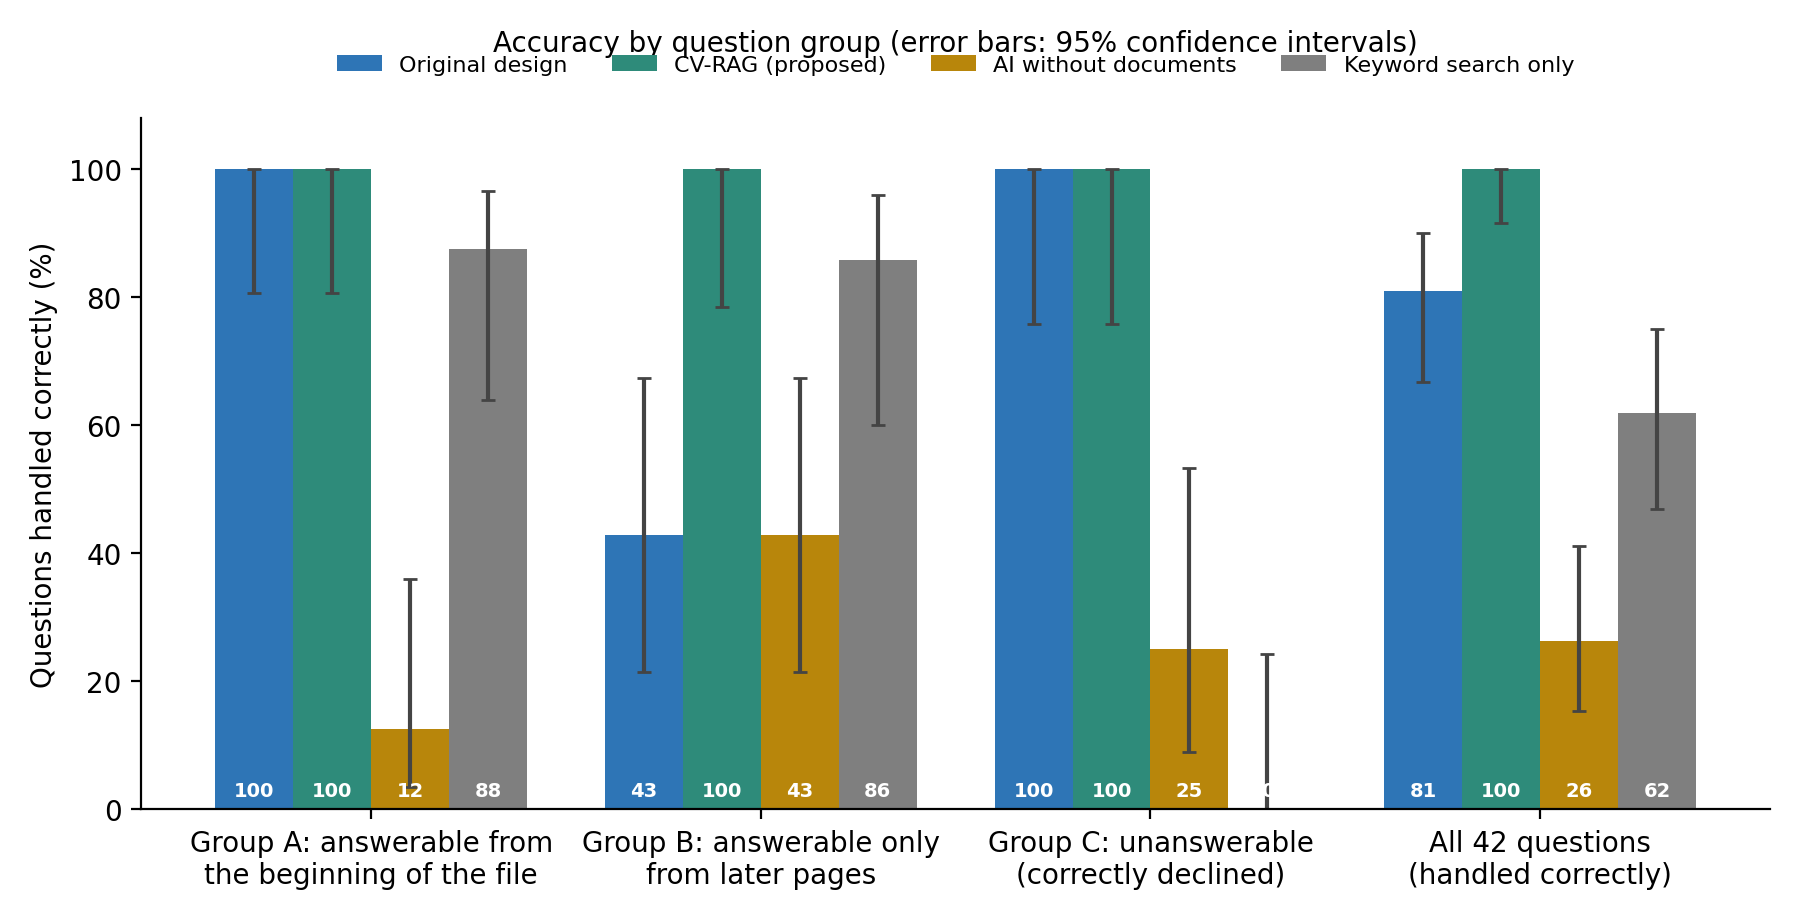
\includegraphics[width=\linewidth]{figures/fig_accuracy_by_split.png}
\caption{Accuracy of each approach by question group (95\% Wilson intervals).}
\label{fig:acc}
\end{figure}

\begin{figure}[t]
\centering
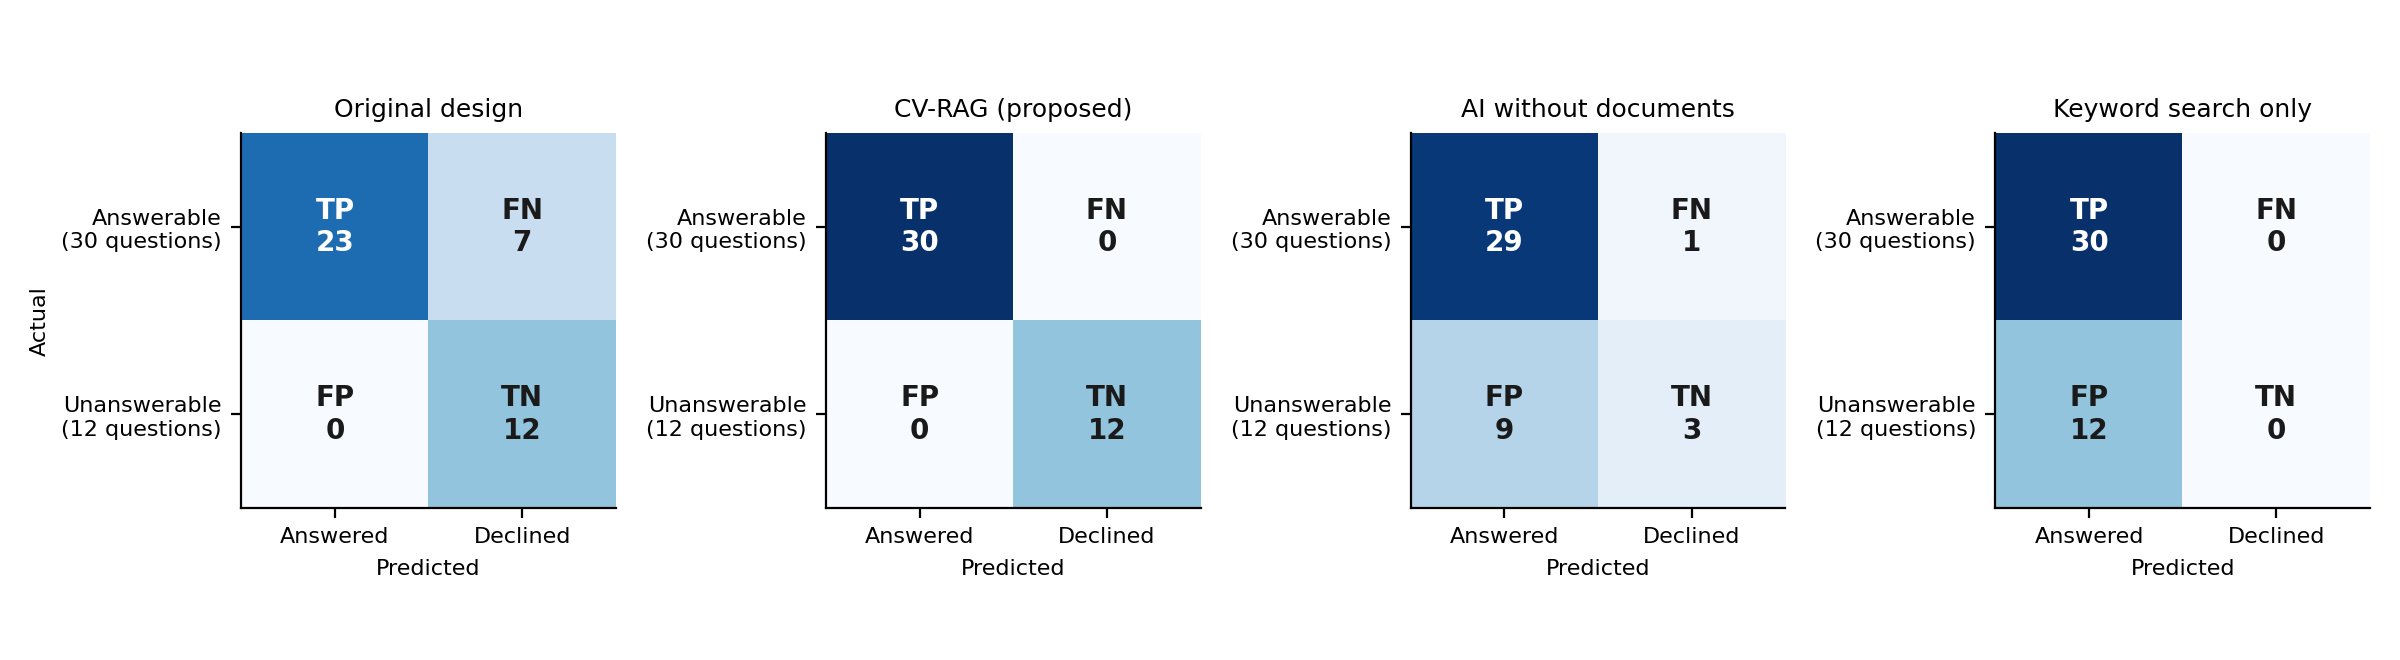
\includegraphics[width=\linewidth]{figures/fig_confusion_matrices.png}
\caption{Confusion matrices of the decision to answer or to decline.}
\label{fig:cm}
\end{figure}

\begin{table}[t]
\centering
\caption{Reading 66 corrupted LLM replies (48 cut off)}
\label{tab:json}
\footnotesize
\begin{tabular}{lccc}
\toprule
\textbf{Method} & \textbf{Read} & \textbf{Cut-off read} & \textbf{Entities rec.}\\
\midrule
Standard JSON & 3 & 0\% & 0\%\\
Fence removal & 9 & 0\% & 0\%\\
Bracket search & 15 & 0\% & 0\%\\
Original partial recovery & 18 & 0\% & 0\%\\
\textbf{Proposed recovery} & \textbf{66} & \textbf{100\%} & \textbf{88\%}\\
\bottomrule
\end{tabular}
\end{table}

To evaluate output recovery, three evidence graphs generated by the LLM for stored cases were altered in 22 realistic ways, including markdown fences, reasoning blocks, explanatory prose and truncation at 30--95\% of the reply, giving 66 inputs. As Table~\ref{tab:json} and Fig.~\ref{fig:json} show, none of the four parsers previously used in the code base could read any of the 48 truncated replies. The proposed method read all 66 and recovered 88\% of graph entities from truncated replies (Cochran's $Q=187.5$, $p<0.001$). Relationships are recovered less often than entities because models write them after the entity list. A functional test of the deployed system revealed the same failure in practice: the trial-brief feature returned template text after its reply was cut off at 1,800 tokens. Generating the brief in three focused requests---chronology, cross-examination bank and synopsis---removed the failure, and all template fallbacks were removed from the platform.

\begin{figure}[t]
\centering
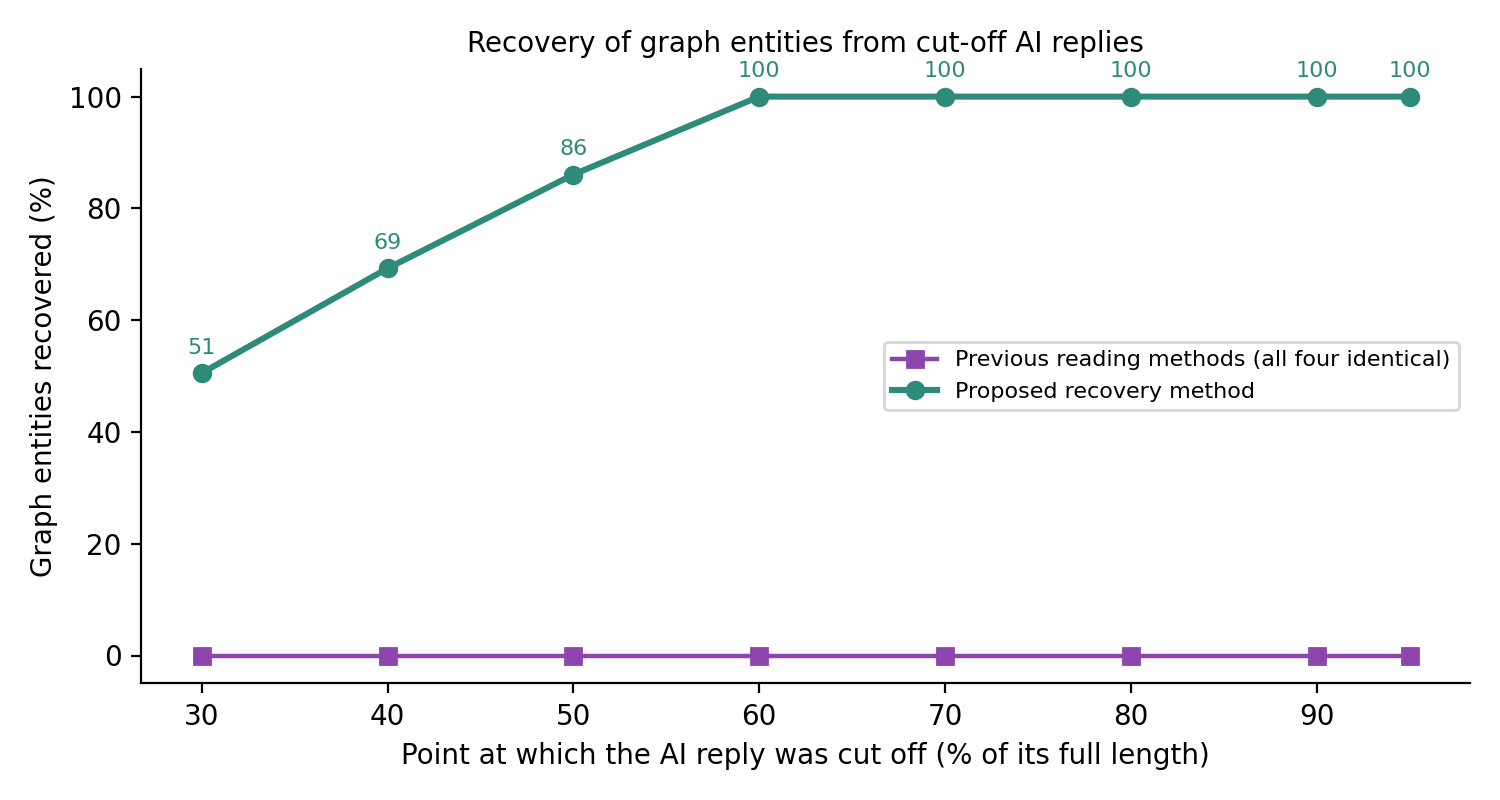
\includegraphics[width=\linewidth]{figures/fig_json_truncation.png}
\caption{Graph entities recovered from LLM replies cut off at different points.}
\label{fig:json}
\end{figure}

%% ----------------------------------------------------------------------------
\section{Limitations}
The question-answering evaluation uses a single judgment and 42 questions with one generation per question, so the confidence intervals are wide and the results should be confirmed on a larger multi-document corpus. Answers were scored automatically against patterns of the known answer, which may accept an answer that also contains unsupported detail; doubtful cases were checked by hand. BM25 matches terms, so questions phrased very differently from the judgment may retrieve weaker passages. At present CV-RAG powers the trial brief, the evidence graph and precedent search, while the chat feature still uses the truncated context. Scanned documents without a text layer are not supported, only English documents were tested, and free-tier rate limits make a full trial brief take one to two minutes.

\section{Conclusion and Future Work}
Court Vision AI shows that a legal case-preparation assistant can be both useful and trustworthy when every output is grounded in the user's own record. The decisive factor in our evaluation was not the model but the information it received: the same LLM moved from 26\% of questions handled correctly without documents, and 81\% with a truncated record, to 100\% with CV-RAG, while using 60\% fewer prompt tokens. Recovering complete objects from cut-off output and removing template fallbacks turned silent failures into correct results or explicit errors, and the precedent library turns every uploaded judgment into a verifiable research resource.

Future work will extend CV-RAG to the chat and courtroom features, combine keyword and semantic retrieval for paraphrased questions, evaluate the system on a multi-document corpus with expert adjudication, conduct a user study with law students and junior advocates, verify AI-suggested citations against public judgment repositories, and add support for scanned documents and Indian languages.

\section*{Acknowledgment}
The authors thank Dr. Asma Praveen for her guidance and the Department of Information Technology, Vivekanand Education Society's Institute of Technology, for its support.

\bibliographystyle{IEEEtran}
\bibliography{refs}

\end{document}
